% Task 7: does S remember the key? CHECKED with python3 and Task7/rc4.py:
%   random.seed(1); key = random.randbytes(16) = 245 177 101 34 74 88 183 145 223 106 241 216 48 62 97 205
%   ksa(key): S[0..7] = 245 42 20 51 237 63 155 72, S[254] = 211, S[255] = 225  (S[0] == key[0])
%   random.seed(4); S = list(range(256)); random.shuffle(S): S[0..7] = 248 196 72 197 126 35 209 214, S[254] = 77, S[255] = 120
%   The two percentages are the result of the task: not shown.
\documentclass[12pt,tikz,border=6pt]{standalone}
% Shared preamble of the task figures of Lecture 1.
% The colours and styles are copied from the preamble of ../main.tex (keep them in sync).
\usepackage{lmodern}
\usepackage[T1]{fontenc}
\renewcommand{\familydefault}{\sfdefault}
\usepackage{amsmath,amssymb}
\usepackage{xcolor}
\usepackage{fontawesome5}
\usetikzlibrary{arrows.meta, calc, positioning, fit, decorations.pathreplacing, decorations.pathmorphing, backgrounds}

% ---------- template ----------
\definecolor{DeepBlue}{HTML}{283593}
\definecolor{AccentOrange}{HTML}{EB5A14}
\definecolor{LightGray}{HTML}{F5F6FA}
% ---------- actors and categories (S1 to S6) ----------
\definecolor{sIndigo}{HTML}{5C6BC0}   % the sender
\definecolor{sPink}{HTML}{EC407A}     % the attacker
\definecolor{sViolet}{HTML}{7E57C2}   % plaintext
\definecolor{sAmber}{HTML}{FFB300}    % key and keystream
\definecolor{sTeal}{HTML}{26A69A}     % the receiver
\definecolor{sBrown}{HTML}{8D6E63}    % ciphertext
\definecolor{sPinkText}{HTML}{C2185B}
\definecolor{sAmberText}{HTML}{A06A00}
\definecolor{sTealText}{HTML}{00796B}
% ---------- actions and results ----------
\definecolor{aExec}{HTML}{43A047}
\definecolor{aRead}{HTML}{1E88E5}
\definecolor{aWrite}{HTML}{E53935}
% ---------- neutral ----------
\definecolor{nInk}{HTML}{37474F}
\definecolor{nLine}{HTML}{90A4AE}
\definecolor{nLight}{HTML}{CFD8DC}
\definecolor{nFill}{HTML}{ECEFF1}
\definecolor{nIdle}{HTML}{E0E0E0}

% ---------- TikZ styles (as in main.tex; byte cells a little larger for the web) ----------
\tikzset{
  hw/.style={draw=nLine, thick, fill=nFill, text=nInk, rounded corners=3pt, align=center, inner sep=4pt},
  hwmain/.style={draw=nInk, thick, fill=nInk, text=white, rounded corners=3pt, align=center, inner sep=4pt},
  cell/.style={draw=nLine, thick, fill=white, text=nInk, font=\ttfamily\small},
  cellfree/.style={cell, dashed, draw=nLight},
  container/.style={draw=nLine, thick, dashed, rounded corners=5pt},
  actor/.style={fill=#1, draw=#1, text=white, rounded corners=3pt, align=center, font=\small\bfseries, inner sep=5pt},
  actorlight/.style={fill=#1!15, draw=#1, thick, text=nInk, rounded corners=3pt, align=center, inner sep=5pt},
  data/.style={-{Stealth}, very thick, nInk},
  flow/.style={-{Stealth}, very thick, DeepBlue},
  annot/.style={draw=AccentOrange, line width=1.6pt, rounded corners=3pt},
  byte/.style={draw=nLine, thick, fill=white, text=nInk, font=\ttfamily\small,
    minimum width=0.8cm, minimum height=0.62cm, inner sep=1pt, rounded corners=1.5pt},
  ptb/.style={byte, fill=sViolet!15, draw=sViolet},
  ksb/.style={byte, fill=sAmber!25, draw=sAmber},
  ctb/.style={byte, fill=sBrown!15, draw=sBrown},
  unk/.style={byte, fill=white, dashed, text=sViolet},
  rowlabel/.style={font=\small\bfseries, text=nInk, anchor=east},
  note/.style={font=\small, text=nInk},
  bigxor/.style={circle, draw=nInk, very thick, fill=white, inner sep=0pt, minimum size=0.8cm, font=\Large},
  radio/.style={-{Stealth}, very thick, nInk, decorate,
    decoration={snake, amplitude=1.2pt, segment length=7pt, post length=4pt}},
  % a white card behind the whole figure, so that it stays readable in a dark theme
  card/.style={show background rectangle, background rectangle/.style={fill=white, draw=none}, inner frame sep=8pt},
}
% a row of bytes: \byterow{x of the first cell}{y}{style}{list of values}{step between cells}
\newcommand{\byterow}[5]{%
  \expandafter\def\expandafter\brlist\expandafter{#4}%
  \foreach \v [count=\k from 0] in \brlist {
    \node[#3] at ({#1+#5*\k},#2) {\v};
  }}
% the generator / cipher box: dark, with cogs. \cogbox{name}{position}{label}{width}
\newcommand{\cogbox}[4]{%
  \node[hwmain, minimum width=#4, minimum height=1.3cm] (#1) at (#2) {};
  \node[text=white, font=\Large] at ([yshift=0.22cm]#1.center) {\faCogs};
  \node[text=white, font=\small\bfseries] at ([yshift=-0.32cm]#1.center) {#3};}
\newcommand{\ok}{\textcolor{aExec}{\faCheck}}
\newcommand{\nok}{\textcolor{aWrite}{\faTimes}}
\newcommand{\badge}[1]{\tikz[baseline=(b.base)]\node[circle,fill=AccentOrange,text=white,
  inner sep=1.5pt,font=\bfseries\footnotesize] (b) {#1};}

\begin{document}
\pagecolor{white}
\begin{tikzpicture}[>=Stealth]
  \def\dx{0.95}
  \def\xs{4.4}
  \tikzset{sc/.style={cell, minimum width=0.8cm, minimum height=0.62cm, rounded corners=1.5pt}}
  % the S table: \stable{y}{8 values}{S[254]}{S[255]}
  \newcommand{\stable}[4]{%
    \byterow{\xs}{#1}{sc}{#2}{\dx}
    \node[text=nInk] at ({\xs+8*\dx},#1) {\ldots};
    \node[sc] at ({\xs+9*\dx},#1) {#3};
    \node[sc] at ({\xs+10*\dx},#1) {#4};}

  % the key
  \node[rowlabel] at ({\xs-0.6},2.4) {key};
  \byterow{\xs}{2.4}{ksb}{245,177,101,34,74,88,183,145,223,106,241,216,48,62,97,205}{\dx}
  \foreach \k in {0,...,15} \node[font=\footnotesize, text=gray] at ({\xs+\dx*\k},2.95) {\k};
  \node[font=\small, text=nInk, anchor=west] at ({\xs-0.4},3.45) {16 random bytes: \texttt{key = random.randbytes(16)}};

  % S after the KSA
  \node[hwmain, minimum width=2.8cm, minimum height=0.8cm, font=\small\bfseries] (ksa) at (1.0,0.8) {\faCogs\ \texttt{ksa(key)}};
  \draw[data] (ksa.east) -- ({\xs-0.55},0.8);
  \node[font=\small\bfseries, text=nInk, anchor=east] at ({\xs-0.6},1.35) {S};
  \foreach \k/\l in {0/0,1/1,2/2,3/3,4/4,5/5,6/6,7/7,9/254,10/255} \node[font=\footnotesize, text=gray] at ({\xs+\dx*\k},1.3) {\l};
  \stable{0.8}{245,42,20,51,237,63,155,72}{211}{225}
  \draw[annot] ({\xs-0.5},0.4) rectangle ({\xs+0.5},2.8);
  \node[font=\small\bfseries, text=AccentOrange, anchor=west] at ({\xs+10.7*\dx},0.8) {\texttt{S[0] == key[0]}: \ \ok\ count it};

  % a fair shuffle
  \node[hw, minimum width=2.8cm, minimum height=0.8cm, font=\small\bfseries, align=center] (sh) at (1.0,-0.6) {\faRandom\ fair shuffle};
  \draw[data] (sh.east) -- ({\xs-0.55},-0.6);
  \stable{-0.6}{248,196,72,197,126,35,209,214}{77}{120}
  \node[font=\small, text=nInk, anchor=west] at ({\xs+10.7*\dx},-0.6) {\texttt{S[0] != key[0]}: \ \nok};
  \node[font=\small, text=gray, anchor=north] at (1.0,-1.05) {\texttt{random.shuffle(S)}};

  % the loop
  \draw[nLight, thick, dashed] (-0.5,-1.75) -- (19.4,-1.75);
  \node[font=\small, text=nInk, anchor=west] at (-0.4,-2.35)
    {\faRedo\ \ Repeat for \textbf{10\,000} random keys. Count both cases:};
  \node[cell, minimum width=4.4cm, minimum height=0.7cm, font=\ttfamily\small] at (12.2,-2.35) {ksa\_hits = ?};
  \node[cell, minimum width=4.4cm, minimum height=0.7cm, font=\ttfamily\small] at (17.2,-2.35) {shuffle\_hits = ?};
  \node[font=\small, text=nInk, anchor=west] at (-0.4,-3.0)
    {Both tables hold every number 0 to 255 once. Does the KSA put \texttt{key[0]} in \texttt{S[0]} more often than a fair shuffle?};
\end{tikzpicture}
\end{document}
